% Intended LaTeX compiler: xelatex
\documentclass[aspectratio=149,11pt]{beamer}
\usepackage{graphicx}
\usepackage{longtable}
\usepackage{wrapfig}
\usepackage{rotating}
\usepackage[normalem]{ulem}
\usepackage{amsmath}
\usepackage{amssymb}
\usepackage{capt-of}
\usepackage{hyperref}
\institute{Università di Siena}
\usepackage{localheader}
\usepackage{tikz}
\usepackage{booktabs,tabularx,tabularray}
\usepackage{setspace}
\usepackage{quoting}
\usepackage[italian]{babel}
\usepackage{fancybox}
\usepackage{tabularray}
\usetheme{default}
\author{Massimo D'Antoni}
\date{2023-2024}
\title{L'analisi normativa dell'intervento pubblico: mercati ed efficienza}
\subtitle{Scienza delle Finanze}
\hypersetup{
 pdfauthor={Massimo D'Antoni},
 pdftitle={L'analisi normativa dell'intervento pubblico: mercati ed efficienza},
 pdflang={Italian}}
\begin{document}

\maketitle

%%%%%%%%%%%%%%%%%%%%%%%%%%%%%%%%%%%%%%%%%%%%
\begin{frame}{Perché l'intervento dello Stato}
\begin{itemize}
\item Alla domanda è possibile rispondere sia da un’ottica positiva che da un’ottica normativa
\begin{itemize}
\item \alert{Positiva}: cosa ha determinato/causato storicamente l’intervento pubblico, perché esso ha assunto una certa forma in uno specifico momento storico. Cosa può determinare un cambiamento di questo ruolo e di queste modalità.
\item \alert{Normativa}: cosa giustifica l’intervento pubblico, in termini di «dover essere».  C’è realmente bisogno di un intervento dello Stato? Qual è il modo migliore per organizzare tale intervento?
\end{itemize}
\item L’assunzione di un’ottica normativa richiede la precisazione di un criterio di valutazione. Quando possiamo ritenere che un esito sia desiderabile? Esiste un interesse della collettività? È responsabilità dello Stato perseguirlo?
\begin{itemize}
\item Tradizionalmente, la risposta a queste domande da parte dell’economia è stata data distinguendo la dimensione dell'\alert{efficienza} da quella dell'\alert{equità}. Entrambi sono obiettivi desiderabili, ma, come vedremo, la definizione di efficienza è più semplice e meno controversa di quella di equità.
\end{itemize}
\end{itemize}
\end{frame}

\section{L'efficienza}


%%%%%%%%%%%%%%%%%%%%%%%%%%%%%%%%%%%%%%%%%%%%
\begin{frame}{Efficienza ed equità}
\begin{itemize}
\item Una premessa non così ovvia: per valutare la bontà di una situazione, una politica, un esito, guardiamo agli \alert{effetti}, alle \alert{conseguenze}, che essa/esso determina per gli individui della collettività.
\item Ricorrendo alla nozione di \alert{efficienza} valutiamo e ordiniamo i diversi esiti senza chiamare in causa i confronti tra individui. Parlando di \alert{equità} ci occupiamo di confrontare e pesare gli effetti sui diversi individui.
\item \alert{Efficienza paretiana} (criterio proposto da Vilfredo Pareto, 1848-1923): è efficiente in senso paretiano e rappresenta un «ottimo paretiano» una situazione data la quale non è possibile migliorare l’utilità di nessuno senza peggiorare quella di qualcun altro
\end{itemize}
\end{frame}

%%%%%%%%%%%%%%%%%%%%%%%%%%%%%%%%%%%%%%%%%%%%
\begin{frame}{Efficienza paretiana}
\begin{itemize}
\item L’efficienza paretiana può essere definita a partire dal criterio di «dominanza paretiana»:
\begin{itemize}
\item A «domina» B (è preferibile in senso paretiano a B) se nessun individuo preferisce B ad A e almeno un individuo preferisce A a B
\item In una versione più debole del criterio: tutti gli individui preferiscono A a B
\end{itemize}
\item Osserviamo che:
\begin{itemize}
\item la seconda versione è più debole in quanto, imponendo criteri più restrittivi per stabilire che A è meglio di B, troverà meno casi nei quali un’alternativa domina un’altra alternativa
\item il criterio è molto parsimonioso in quanto non richiede alcuna informazione sull’intensità delle preferenze dei diversi individui
\end{itemize}
\item Un esito è efficiente se non è dominato da altri esiti tra quelli disponibili.
\begin{itemize}
\item N.B. Date le preferenze degli individui, un esito può cessare di essere efficiente se aumentiamo l’insieme di esiti disponibili, può diventare efficiente se riduciamo tale insieme
\end{itemize}
\end{itemize}
\end{frame}

%%%%%%%%%%%%%%%%%%%%%%%%%%%%%%%%%%%%%%%%%%%%
\begin{frame}{Un esempio: individuiamo gli esiti efficienti}
\begin{columns}
\begin{column}{.5\columnwidth}
\begin{itemize}
\item Consideriamo 5 possibili esiti e due individui:
\begin{itemize}
\item Individuo 1: A > B > C > D > E
\item Individuo 2: E > B > C > A > D
\end{itemize}
\item Verifichiamo se un esito è dominato, cioè se esiste un altro esito ad esso preferito da entrambi gli individui.
\item Un esito non dominato è efficiente.
\item In questo caso, gli esiti C e D sono dominati da altri esiti
\item Gli esiti efficienti sono E, B e A.
\end{itemize}
\end{column}

\begin{column}{.5\columnwidth}
\footnotesize
Potremmo assegnare dei valori numerici 
coerenti con gli ordinamenti e rappresentare
le opzioni graficamente:

\begin{center}
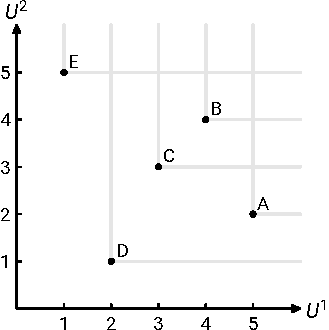
\includegraphics[width=\textwidth]{./figure/efficienza-1.pdf}
\end{center}
\end{column}
\end{columns}
\end{frame}

%%%%%%%%%%%%%%%%%%%%%%%%%%%%%%%%%%%%%%%%%%%%
\begin{frame}{Alcune osservazioni sulla nozione di efficienza}
\begin{itemize}
\item La popolarità del concetto di efficienza deriva dal fatto che la bontà di un miglioramento paretiano non richiede confronti interpersonali
\item Una tradizione molto influente nell’economia politica del XIX secolo è stato l’utilitarismo, per il quale è desiderabile ciò che aumenta l’utilità complessiva di una collettività. Nell’ambito dell’utilitarismo era concettualmente possibile confrontare l’aumento di utilità di un individuo con la riduzione dell’utilità di un altro individuo.
\item A partire dagli anni ‘30 del XX secolo, si è affermata una visione critica, che ha rifiutato l’idea che l’utilità fosse confrontabile. L’utilità è uno stato mentale degli individui non osservabile.
\item Se l’economia deve basarsi su ciò che è osservabile, al massimo posso stabilire che un individuo preferisce l’opzione A all’opzione B in quanto, posto di fronte a entrambe le opzioni, sceglie la prima.
\item Non posso invece rispondere a domande come «quanto è intensa la preferenza di A rispetto a B per l’individuo 1 se confrontata con la preferenza di B rispetto ad A dell’individuo 2?»
\end{itemize}
\end{frame}

%%%%%%%%%%%%%%%%%%%%%%%%%%%%%%%%%%%%%%%%%%%%
\begin{frame}{Alcune osservazioni sulla nozione di efficienza /2}
\begin{itemize}
\item Il criterio paretiano consente di effettuare confronti basandosi esclusivamente sulla conoscenza del fatto che per un ciascun individuo A è meglio/peggio di B
\item Si tratta di un criterio che, quando rispettato, risulta coerente con altri più esigenti criteri:
\begin{itemize}
\item il criterio della maggioranza: se A è Pareto superiore a B, allora A sarà preferito a B a maggioranza
\item il criterio utilitarista: se A è Pareto superiore a B, vuol dire che l’utilità di tutti gli individui aumenta (o non diminuisce), quindi anche l’utilità totale aumenta
\end{itemize}
\item Ovviamente, ci sono molti casi nei quali il criterio non ci fornisce una risposta, anche quando a noi tale risposta appare ovvia:
\item Se una politica toglie 100€ a un individuo povero per aumentare di 10€ il reddito di un individuo ricco, sulla base del criterio paretiano non siamo in grado di dire che tale politica non è desiderabile
\item Cosa dire del caso in cui diamo 1000€ a un individuo ricco e non diamo nulla ad altri individui più poveri?
\end{itemize}
\end{frame}

%%%%%%%%%%%%%%%%%%%%%%%%%%%%%%%%%%%%%%%%%%%%
\begin{frame}{L'efficienza potenziale e il test di compensazione}
\begin{itemize}
\item Supponiamo di considerare un cambiamento dello status quo che determina un vantaggio considerevole per un numero elevato di individui al prezzo di uno svantaggio modesto per pochi individui (al limite uno solo).
\begin{itemize}
\item Il cambiamento non è un miglioramento paretiano
\item \ldots{}eppure ci appare desiderabile!
\end{itemize}
\item Kaldor e Hicks negli anni '30 del XX secolo hanno proposto di uscire da questa impasse immaginando un’ipotetica compensazione monetaria tra «vincenti» e «perdenti» a seguito del cambiamento.
\item Il criterio da loro individuato effettua un confronto tra guadagni e perdite quantificandoli in termini monetari
\end{itemize}
\end{frame}


%%%%%%%%%%%%%%%%%%%%%%%%%%%%%%%%%%%%%%%%%%%%
\begin{frame}{L'efficienza potenziale e il test di compensazione /2}
\begin{itemize}
\item Nella versione di Kaldor:
\begin{itemize}
\item Chiediamo ai perdenti quale somma monetaria potrebbe compensarli dell’adozione del cambiamento proposto
\item Chiediamo ai vincenti se essi continuerebbero a desiderare il cambiamento anche qualora dovessero pagare ai perdenti una compensazione pari alla cifra da questi indicata
\item Se la risposta è positiva, il cambiamento supera il test ed è socialmente desiderabile
\end{itemize}
\item Nella versione di Hicks:
\begin{itemize}
\item Chiediamo ai vincenti quale somma monetaria potrebbe compensarli della mancata adozione del cambiamento proposto
\item Chiediamo ai perdenti se essi sarebbero disposti a pagare la somma indicata dai vincenti per evitare il cambiamento che li danneggia
\item Se la risposta è negativa, il cambiamento supera il test ed è socialmente desiderabile
\end{itemize}
\end{itemize}
\end{frame}

%%%%%%%%%%%%%%%%%%%%%%%%%%%%%%%%%%%%%%%%%%%%
\begin{frame}{Il test di compensazione in formule}
\begin{itemize}
\item In formule:
\begin{itemize}
\item Poniamo che l’utilità di i dipenda da una certa azione del governo e dal
reddito $U^i(X, R^i)$, dove $X\in\{A, B\}$,
\item se nel passaggio da B ad A l’individuo 1 è un vincente e l’individuo 2 è
un perdente abbiamo:
$U^1(A, R^1) > U^1(B, R^1)$ e $U^2(A, R^2) < U^2(B, R^2)$
\item esisteranno dunque due somme $Y^1$ e $Y^2$ (dette variazioni compensative) tali che
\begin{equation*}
U^1(A, R - Y^1) = U^1(B, R^1) \qquad U^2(A, R + Y^2) = U^2(B, R^2)
\end{equation*}
\item il test di Kaldor è soddisfatto se $Y^1 >  Y^2$
\end{itemize}
\item Trovate le formule corrispondenti per il criterio di Hicks, che utilizza le
variazioni equivalenti
\item I due criteri differiscono perché la somma che sono disposto a pagare per
ottenere un cambiamento che mi avvantaggia non coincide in generale con la
somma che sono disposto ad accettare per rinunciarvi (le variazioni
compensative e le variazioni equivalenti non coincidono)
\end{itemize}
\end{frame}

%%%%%%%%%%%%%%%%%%%%%%%%%%%%%%%%%%%%%%%%%%%%
\begin{frame}{Il test di compensazione: osservazioni}
\begin{itemize}
\item Il test di compensazione non richiede che la compensazione abbia effettivamente luogo (se così fosse saremmo in presenza di un miglioramento paretiano). È sufficiente che essa sia \alert{ipoteticamente} possibile.
\begin{itemize}
\item Se la valutazione non ha luogo, a essere svantaggiato potrebbe essere un individuo con reddito più basso
\item Ci convince come criterio di valutazione?
\end{itemize}
\item Proprio perché variazioni equivalenti e compensative non sono uguali, A potrebbe essere meglio di B secondo Kaldor (Hicks) ma non secondo Hicks (Kaldor)
\item Possono anche aver luogo dei paradossi: 
\begin{itemize}
\item Potrebbe accadere che, secondo uno dei due criteri, A è meglio di B e contemporaneamente B è meglio di A!
\end{itemize}
\end{itemize}
\end{frame}

%%%%%%%%%%%%%%%%%%%%%%%%%%%%%%%%%%%%%%%%%%%%
\begin{frame}{L'efficienza potenziale nell'analisi economica}
\begin{itemize}
\item Quando gli economisti parlano di una soluzione «più efficiente», spesso fanno riferimento all’efficienza potenziale più che all’efficienza paretiana.
\item Essi intendono dire che si è determinata una situazione a partire dalla quale, con un opportuno schema di trasferimenti monetari, è possibile ottenere un miglioramento paretiano.
\item Potremmo dire che l’efficienza viene intesa come la massimizzazione del valore creato da una certa politica o una certa azione, un valore misurato in termini di variazioni monetarie equivalenti o compensative
\item In questo modo, si separano le considerazioni di efficienza (la «dimensione della torta» aumenta) da quelle equitative (come la maggiore torta viene divisa tra le parti). Si rimanda implicitamente la determinazione degli effetti redistributivi a un momento logicamente (e temporalmente) successivo.
\end{itemize}
\end{frame}
\section{Efficienza e mercati nel modello neoclassico}

%%%%%%%%%%%%%%%%%%%%%%%%%%%%%%%%%%%%%%%%%%%%
\begin{frame}{L'efficienza in un'economia di beni privati}
\begin{itemize}
\item \alert{Beni privati} = è possibile escludere altri dal consumo (escludibilità) e il
mio consumo rende impossibile il consumo dello stesso bene da parte di altri
(rivalità)
\begin{itemize}
\item La rivalità implica: $X = x^1 + x^2 + \dots + x^n$
\end{itemize}
\item Un esito è un'\alert{allocazione}, cioè una descrizione di quanto ciascun individuo
consuma di ciascun bene.
\item Se nell’economia non c’è produzione (economia di «puro scambio») possiamo
rappresentare tutte le possibili allocazioni come punti contenuti in un
rettangolo, la «scatola di Edgeworth»
\end{itemize}
\end{frame}

%%%%%%%%%%%%%%%%%%%%%%%%%%%%%%%%%%%%%%%%%%%%
\begin{frame}{Allocazioni efficienti nella scatola di Edgeworth}
\begin{columns}
\begin{column}{.5\columnwidth}
\fontsize{11}{11}\selectfont
\begin{itemize}
\item 2 individui (1 e 2) e 2 beni (X e Y)
\item Nella scatola di Edgeworth possiamo tracciare le curve di indifferenza dei due individui passanti per un punto/allocazione. Esse individuano le allocazioni preferite all’allocazione di partenza.
\item A meno che le curve di indifferenza siano tangenti, l’allocazione è inefficiente in quanto dominata da allocazioni preferite da entrambi (es. allocazione B).
\item La condizione di tangenza delle curve di indifferenza caratterizza dunque le allocazioni efficienti (es. allocazione A)
\end{itemize}
\end{column}
\begin{column}{.5\columnwidth}
\footnotesize
Formalmente la condizione di tangenza
tra curve di indifferenza: $\text{SMS}^1_{XY}=\text{SMS}^2_{XY}$

\begin{figure}
\centering
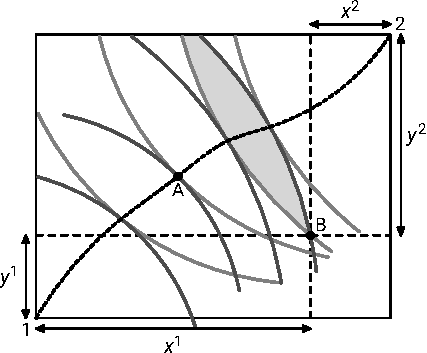
\includegraphics[height=4cm]{./figure/edgeworth-1.pdf}
\end{figure}

Il saggio marginale di sostituzione (SMS) rappresenta l’inclinazione della curva di indifferenza. 
\end{column}
\end{columns}
\end{frame}

%%%%%%%%%%%%%%%%%%%%%%%%%%%%%%%%%%%%%%%%%%%%
\begin{frame}{Allocazioni efficienti nella scatola di Edgeworth /2}
\begin{columns}
\begin{column}{.5\columnwidth}
\begin{figure}
\centering
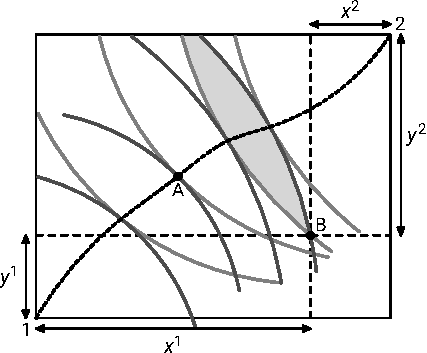
\includegraphics[height=5cm]{./figure/edgeworth-1.pdf}
\end{figure}
\end{column}

\begin{column}{.5\columnwidth}
\begin{itemize}
\item La soluzione efficiente realizza il massimo di utilità di un individuo data l’utilità dell’altro individuo.
\item Ci sono infinite allocazioni efficienti (sulla «curva dei contratti»).
\item Spostandosi da una allocazione efficiente all’altra si migliora la condizione di uno dei due individui a spese dell’altro.
\item Nota bene: nell’esempio, l’allocazione efficiente A non è Pareto superiore all’allocazione inefficiente B
\end{itemize}
\end{column}
\end{columns}
\end{frame}

%%%%%%%%%%%%%%%%%%%%%%%%%%%%%%%%%%%%%%%%%%%%
\begin{frame}{Un'economia con produzione}
\begin{columns}
\begin{column}{.5\columnwidth}
\begin{itemize}
\item Nel caso più semplice: un input (lavoro, L) che può essere allocato alla
produzione di due beni X e Y:
\begin{equation*}
X = f_X(L_X)\quad  Y = f_Y(L_Y)\quad L = LX + LY
\end{equation*}
\item La frontiera, che rappresenta le combinazioni efficienti (\alert{frontiera delle
possibilità di produzione}), è concava per effetto dell’ipotesi di rendimenti
decrescenti
\item L’inclinazione della frontiera è il SMT (\alert{saggio marginale di trasformazione})
il SMT è pari al rapporto tra i costi marginali di produzione dei due beni
\begin{equation*}
\text{SMT}_{XY}=\frac{\text{CMg}_X}{\text{CMg}_Y}
\end{equation*}
\end{itemize}
\end{column}


\begin{column}{.5\columnwidth}
\begin{figure}[htbp]
\centering
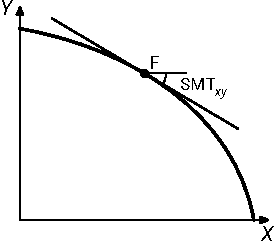
\includegraphics[height=5cm]{./figure/frontiere-1.pdf}
\end{figure}
\end{column}
\end{columns}
\end{frame}

%%%%%%%%%%%%%%%%%%%%%%%%%%%%%%%%%%%%%%%%%%%%
\begin{frame}{Efficienza con produzione}
\begin{columns}
\begin{column}{.5\columnwidth}
\begin{itemize}
\item L’efficienza nello scambio e nella produzione è individuata dalla condizione:
\begin{equation*}
\text{SMT}^1_{XY}=\text{SMT}^2_{XY}=\text{SMT}_{XY}
\end{equation*}
\end{itemize}
\end{column}

\begin{column}{.5\columnwidth}
\begin{figure}[htbp]
\centering
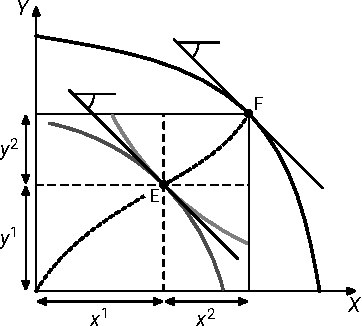
\includegraphics[height=5cm]{./figure/edgeworth-2.pdf}
\end{figure}
\end{column}
\end{columns}
\end{frame}

%%%%%%%%%%%%%%%%%%%%%%%%%%%%%%%%%%%%%%%%%%%%
\begin{frame}{Frontiera del benessere}
\begin{columns}
\begin{column}{.5\columnwidth}
\begin{itemize}
\item Date le risorse disponibili e la tecnologia
\item fissato un livello minimo di utilità per un individuo ($U^2$)
\item la soluzione efficiente individua il massimo livello di utilità ottenibile dall’altro individuo ($U^1$)
\item Ci sono dunque molteplici soluzioni efficienti, una per ciascun livello $U^2$
\item Le combinazioni di utilità dei due individui così determinate individuano la cosiddetta \alert{frontiera del benessere}
\end{itemize}
\end{column}
\begin{column}{.5\columnwidth}
\begin{figure}[htbp]
\centering
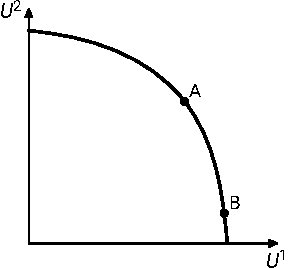
\includegraphics[height=5cm]{./figure/frontiere-2.pdf}
\end{figure}
\end{column}
\end{columns}
\end{frame}

\section{I teoremi fondamentali dell'economia del benessere}


%%%%%%%%%%%%%%%%%%%%%%%%%%%%%%%%%%%%%%%%%%%%
\begin{frame}{Primo teorema fondamentale dell’economia del benessere}
Supponiamo che:
\begin{itemize}
\item tutte le interazioni avvengono su mercati concorrenziali;
\item l’utilità degli individui è determinata esclusivamente dal consumo dai beni
acquistati sui mercati;
\item mercati concorrenziali = gli individui sono price taker, non hanno la
possibilità di influenzare i prezzi con le loro decisioni;
\item sulla base dei prezzi di mercato gli individui formulano i propri piani di
consumo (e quindi di acquisto/vendita);
\item il mercato rende compatibili tali piani: i prezzi di mercato si modificano
fino ad eguagliare domanda e offerta di ciascun bene.
\end{itemize}
\begin{block}{}
L’allocazione ottenuta in corrispondenza di un equilibrio di mercato concorrenziale è efficiente in senso paretiano (o anche: rappresenta un ottimo paretiano).
\end{block}
\end{frame}


%%%%%%%%%%%%%%%%%%%%%%%%%%%%%%%%%%%%%%%%%%%%
\begin{frame}{Primo teorema fondamentale dell’economia del benessere /2}
\begin{columns}
\begin{column}{.5\columnwidth}
In un equilibrio di mercato concorrenziale le curve di indifferenza degli individui sono tangenti

\begin{figure}[htbp]
\centering
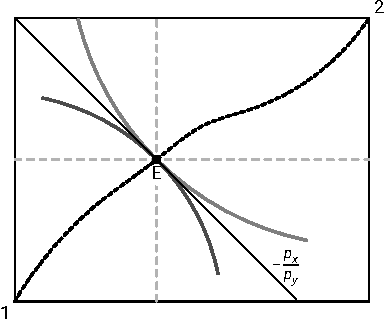
\includegraphics[height=5cm]{./figure/edgeworth-4.pdf}
\end{figure}
\end{column}

\begin{column}{.5\columnwidth}
\begin{figure}[htbp]
\centering
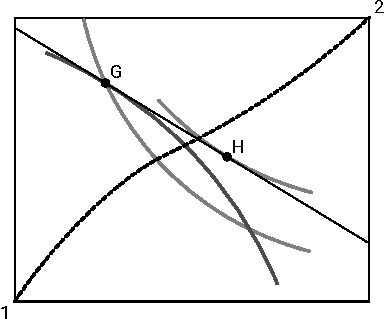
\includegraphics[height=5cm]{./figure/edgeworth-5.pdf}
\end{figure}
\small
In G, dove le curve di indifferenza sono tangenti, non può esserci equilibrio di mercato concorrenziale: se i prezzi rendono ottimo G per 2, l’ottimo per 1 è in H
\end{column}
\end{columns}
\end{frame}

%%%%%%%%%%%%%%%%%%%%%%%%%%%%%%%%%%%%%%%%%%%%
\begin{frame}{Una spiegazione intuitiva del I teorema fondamentale}
\begin{itemize}
\item Un altro modo per illustrare il risultato del I teorema, utilizzando le condizioni al margine:
\begin{itemize}
\item Se gli individui sono \emph{price taker}, fisserano il paniere ottimale in corrispondenza del punto in cui
\end{itemize}
\begin{equation*}
\text{SMS}^1_{XY}=\frac{p_X}{p_Y} \qquad \text{SMS}^2_{XY}=\frac{p_X}{p_Y}
\end{equation*}
\begin{itemize}
\item Se tutti scambiano sulla base degli stessi prezzi:
\end{itemize}
$\text{SMS}^1_{XY} = \text{SMS}^2_{XY}$
\item considerando anche la produzione:
\begin{itemize}
\item un’impresa concorrenziale fissa la propria quantità in corrispondenza del punto in cui:   $\text{CMg}_X=p_X$
\item da cui: $$\text{SMT}_{XY}=\frac{\text{CMg}_X}{\text{CMg}_Y}=\frac{p_X}{p_Y} = \text{SMS}^i_{XY}$$
\end{itemize}
\end{itemize}
\end{frame}

%%%%%%%%%%%%%%%%%%%%%%%%%%%%%%%%%%%%%%%%%%%%
\begin{frame}{La rilevanza pratica del I teorema fondamentale}
\begin{itemize}
\item Il teorema formalizza quanto già Adam Smith aveva teorizzato con la metafora
della «mano invisibile»: le scelte decentrate degli individui, coordinate
attraverso i mercati concorrenziali, garantiscono un ottimo uso delle
risorse
\item Nel chiarire questa conclusione, il teorema evidenzia le condizioni
necessarie perché questa conclusione sia valida. Condizioni di validità del
teorema sono:
\begin{itemize}
\item la presenza di beni che non hanno le caratteristiche di beni privati
(rivalità ed escludibilità)
\item l’assenza di \alert{concorrenza}
\item la presenza di interazioni che non passano attraverso i mercati (le
\alert{esternalità})
\item la rinuncia a scambi mutuamente vantaggiosi per effetto della presenza di
\alert{asimmetrie informative}.
\end{itemize}
\item Si tratta di casi nei quali, diversamente da quanto previsto dal teorema, il
mercato non garantisce un esito efficiente («fallimenti del mercato»).
\item Quanto sono diffusi i casi di fallimento del mercato?
\end{itemize}
\end{frame}

%%%%%%%%%%%%%%%%%%%%%%%%%%%%%%%%%%%%%%%%%%%%
\begin{frame}{Secondo teorema fondamentale dell'economia del benessere}
\begin{block}{}
Sotto ipotesi di convessità delle preferenze e della tecnologia, qualsiasi allocazione efficiente è ottenibile come equilibrio di mercato. 
\end{block}
\begin{itemize}
\item Presa una qualsiasi allocazione efficiente E, esiste un insieme di prezzi e
una distribuzione iniziale delle risorse tali che l’allocazione di
equilibrio è E.
\item Dunque, non solo gli equilibri di mercato concorrenziale sono un
sottoinsieme dell’insieme delle allocazioni efficienti (come afferma il I
teorema). Il teorema afferma che ogni elemento dell’insieme degli
ottimi paretiani è ottenibile come equilibrio di mercato.
\end{itemize}
\end{frame}


%%%%%%%%%%%%%%%%%%%%%%%%%%%%%%%%%%%%%%%%%%%%
\begin{frame}{Secondo teorema fondamentale dell'economia del benessere /2}
\begin{columns}
\begin{column}{.45\columnwidth}
\begin{itemize}
\item Potremmo riformularlo dicendo che: data una qualsiasi allocazione efficiente E e una qualsiasi distribuzione iniziale delle risorse A, è sempre possibile, effettuando un opportuno trasferimento di risorse, arrivare a un equilibrio di mercato concorrenziale che realizza E.
\item Per raggiungere E non c’è necessità di interferire con il meccanismo dei prezzi, basta un trasferimento, da effettuarsi «a monte» del sistema di mercato
\end{itemize}
\end{column}

\begin{column}{.55\columnwidth}
\begin{figure}
\centering
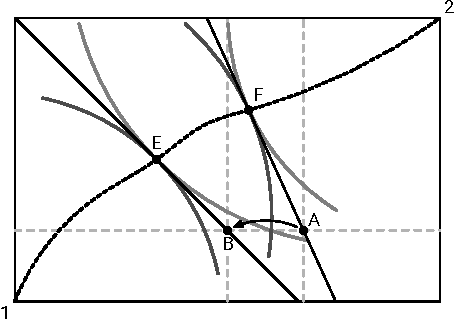
\includegraphics[height=5cm]{./figure/edgeworth-6.pdf}
\end{figure}
\end{column}
\end{columns}
\end{frame}


%%%%%%%%%%%%%%%%%%%%%%%%%%%%%%%%%%%%%%%%%%%%
\begin{frame}{Secondo teorema fondamentale: l'ipotesi di convessità}
\begin{columns}
\begin{column}{.45\columnwidth}
\small
\begin{itemize}
\item Il secondo teorema può apparire ovvio, ma la condizione sulla convessità delle preferenze e della tecnologia mostra che in alcuni casi una soluzione efficiente potrebbe non essere ottenibile come equilibrio di mercato
\item Nella figura, abbiamo ipotizzato preferenze non convesse per l’individuo 1
\item L’allocazione E è efficiente, ma non esistono prezzi in grado di ottenere tale allocazione come equilibrio di mercato (ai prezzi che rendono ottimale la scelta di E per 2, l’individuo 1 sceglierà F)
\end{itemize}
\end{column}

\begin{column}{.55\columnwidth}
\begin{figure}
\centering
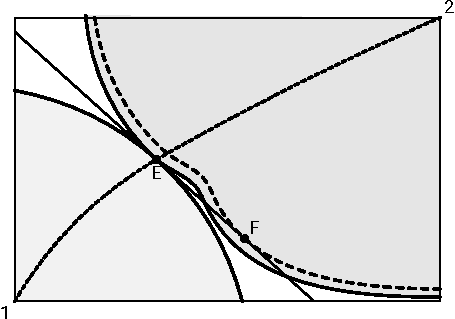
\includegraphics[height=5cm]{./figure/edgeworth-7.pdf}
\end{figure}
\end{column}
\end{columns}
\end{frame}


%%%%%%%%%%%%%%%%%%%%%%%%%%%%%%%%%%%%%%%%%%%%
\begin{frame}{La rilevanza pratica del II teorema fondamentale}
\begin{itemize}
\item Qual è l’effettiva portata del secondo teorema fondamentale?
\item Il trasferimento di risorse, per consentire al mercato di conseguire
l’efficienza, dovrebbe avvenire senza interferire con il sistema dei prezzi
\item Tuttavia, è difficile immaginare modalità di trasferimento con questa caratteristica
\item L’imposta «ideale» da questo punto di vista è un’imposta il cui ammontare
non dipende dalle decisioni individuali. Ovvero un’imposta in somma fissa
(\emph{lump sum tax}).
\item Nessuna imposta «reale» ha le caratteristiche di un’imposta in somma
fissa. Nella realtà è difficile individuare qualcosa di analogo alle
«dotazioni iniziali» del modello di equilibrio economico generale, cui
commisurare le imposte.
\item Il secondo teorema fondamentale, come anche il primo, va inteso come una
\alert{costruzione astratta e ideale}, che individua le condizioni per un’ideale
separazione tra la dimensione dell’efficienza (lasciata al mercato) e quella
dell’equità (responsabilità dello Stato)
\end{itemize}
\end{frame}

%%%%%%%%%%%%%%%%%%%%%%%%%%%%%%%%%%%%%%%%%%%%
\begin{frame}{A sua volta l'intervento dello Stato non è esente da problemi}
\begin{itemize}
\item L'azione di governo, anche quando ben orientata, soffre le conseguenze di
limitazioni informative;
\item i limiti dei meccanismi di scelta collettiva possono portare a decisioni che
non riflettono in modo adeguato le preferenze dei membri della collettività;
\item chi deve eseguire le decisioni pubbliche potrebbe perseguire obiettivi
diversi da quelli della collettività;
\item gli attori economici possono distogliere risorse dalle attività produttive e
impiegarle per condizionare a proprio favore l’azione del governo (\emph{rent
seeking});
\item l'azione del governo può interferire negativamente con l'azione del mercato,
provocando distorsioni e inefficienze
\begin{itemize}
\item ESEMPIO: le imposte e i sussidi necessari per realizzare una più equa
distribuzione possono scoraggiare l'attività economica
\end{itemize}
\end{itemize}
\end{frame}

%%%%%%%%%%%%%%%%%%%%%%%%%%%%%%%%%%%%%%%%%%%%
\begin{frame}{La giustificazione dell'intervento pubblico: una sintesi}
\begin{itemize}
\item L'analisi economica ci spiega come il mercato sia in grado di coordinare in
modo efficiente l'attività economica degli individui, fornendo incentivi e
guidandone le scelte (la «mano invisibile»)
\item Il mercato come meccanismo di organizzazione sociale è insufficiente e non
vive nel vuoto istituzionale: è necessario un quadro di norme e garanzia di
esercizio dei diritti di proprietà
\item \alert{«Fallimenti del mercato»}: circostanze in cui l'esito del mercato non è
efficiente e può (almeno astrattamente) essere migliorato da un intervento
correttivo dello Stato:
\begin{itemize}
\item esternalità
\item beni «pubblici», che il mercato non garantisce in quantità adeguata
\item mercati non concorrenziali (in particolare: monopoli naturali)
\item mercati incompleti o mancanti (in particolare: mercati assicurativi,
mercati con asimmetrie informative)
\end{itemize}
\item Il mercato non garantisce l'\alert{equità distributiva}.
\end{itemize}
\end{frame}
\end{document}